% 包含ctexbeamer文档类
\documentclass[aspectratio=43, xcolor=svgnames, t, 10pt]{beamer}
\usepackage{ctex}
\usepackage{booktabs}%用于制作三线表
\mode<presentation>
% \documentclass[aspectratio=169]{beamer}
% Sets aspect ratio to 16:9, and frame size to 160mm by 90mm.
% \documentclass[aspectratio=43]{beamer}
% The default aspect ratio and frame size. You need not specify this option.

%% 输出绘制有文档线条的笔记区
% \pgfpagesuselayout{4 on 1 with notes}[a4paper,border shrink=5mm]
%\pgfpagesuselayout{1 on 1 with notes landscape}[a4paper, border shrink=5mm]
%\pgfpagesuselayout{2 on 1 with notes}[a4paper,border shrink=5mm]
%\pgfpagesuselayout{3 on 1 with notes}[a4paper,border shrink=5mm]
%\pgfpagesuselayout{2 on 1 with notes landscape}[a4paper,border shrink=5mm]
%\pgfpagesuselayout{1 on 1 with notes}[a4paper,border shrink=5mm]
%%errors dont know why


% 载入需要的宏包
% 加载宏包
%===================注意======================%
% 在调用beamer.cls宏包后,以下宏包将自动调用,
% 不应单独调用这些宏包,以免发生冲突
% amsfonts, amsmath, amssymb, amsthm, 
% enumerate, geometry, graphics, graphicx, 
% hyperref, url, 
% ifpdf, keyval, xcolor, xxcolor
% =============================================%


% 叉号与对号要用到的字体
\usepackage{pifont}

% 生成笔记区的宏包
\usepackage{handoutWithNotes}


%%% Local Variables: 
%%% mode: latex
%%% TeX-master: "../main.tex"
%%% End:


% 进行必要的设置
\usetheme[
%%% 外部主题选项
%    hidetitle,           % 隐藏边栏中的短标题
%    hideauthor,          % 隐藏边栏中的作者缩写
%    hideinstitute,       % 隐藏边栏底部的单位缩写
    shownavsym,          % 显示导航符号
    width=1.5cm,           % 边栏宽度 (默认是 2 cm)
%    hideothersubsections,% 除了当前section的subsection隐藏其它所有 subsections
%    hideallsubsections,  % 隐藏所有 subsections
    left,               % 边栏位置 (默认在右边)
%%% 颜色主题选项
    %lightheaderbg       % 页眉背景颜色
  ]{NWSUAFsidebar}

% 如果需要更改主题中不同元素的颜色,请取消相应注释并编辑为喜欢的颜色
% 分割条和边栏颜色:
%\setbeamercolor{NWSUAFsidebar}{fg=red!20,bg=red}
%\setbeamercolor{sidebar}{bg=red!20}
% 结构元素颜色:
%\setbeamercolor{structure}{fg=red}
% 帧标题颜色:
%\setbeamercolor{frametitle}{fg=blue!25}
% 正文文本背景色:
%\setbeamercolor{normal text}{bg=gray!10}
% ... 如果需要更改更多的参数,请参考 beamer 用户手册.
% \setbeamertemplate{blocks}[default]

\definecolor{Descitem}{RGB}{0, 0, 139}

\definecolor{StdTitle}{RGB}{26, 33, 141}
\definecolor{StdBody}{RGB}{213,24,0}

\definecolor{AlTitle}{RGB}{255, 190, 190}
\definecolor{AlBody}{RGB}{213,24,0}

\definecolor{ExTitle}{RGB}{201, 217, 217}
\definecolor{ExBody}{RGB}{213,24,0}



\definecolor{bananayellow}{rgb}{1.0, 0.88, 0.21}
\definecolor{arylideyellow}{rgb}{0.91, 0.84, 0.42}
\definecolor{forestgreen}{rgb}{0.13, 0.55, 0.13}
\definecolor{mordantred19}{rgb}{0.68, 0.05, 0.0}
\definecolor{amber}{rgb}{1.0, 0.75, 0.0}
\definecolor{blue}{rgb}{0.0, 0.0, 1.0}
\definecolor{corn}{rgb}{0.98, 0.93, 0.36}

% Standard block
\setbeamercolor{block title}{fg = Descitem, bg = StdTitle!15!white}
\setbeamercolor{block body}{bg = StdBody!5!white}
% Alert block
\setbeamercolor{block title alerted}{fg = Descitem, bg = AlTitle}
\setbeamercolor{block body alerted}{bg = AlBody!5!white}
% Example block
\setbeamercolor{block title example}{bg = ExTitle}
\setbeamercolor{block body example}{bg = ExBody!5!white}

\setbeamerfont{block title}{size=\scriptsize}
\setbeamertemplate{blocks}[rounded][shadow=true]
\setbeamertemplate{section in toc}[sections numbered]
% \setbeamercolor{section number projected}{bg=black,fg=yellow}
% \setbeamercolor{section in toc}{color=black}
% 不需要导向条符号
%\beamertemplatenavigationsymbolsempty
\setbeamertemplate{navigation symbols}{}

% block environment whose can be adjusted
\newenvironment<>{varblock}[2][.9\textwidth]{%
  \setlength{\textwidth}{#1}
  \begin{actionenv}#3%
    \def\insertblocktitle{#2}%
    \par%
    \usebeamertemplate{block begin}}
  {\par%
    \usebeamertemplate{block end}%
  \end{actionenv}}
%% 自定义相关的名称宏命令
%% ==================================================
%% \newcommand{\yourcommand}[参数个数]{内容}
% 西北农林科技大学各单位名称
\newcommand{\nwsuaf}{西北农林科技大学}
\newcommand{\cie}{信息工程学院}
\newcommand{\ca}{农学院}
\newcommand{\cpp}{植物保护学院}
\newcommand{\ch}{园艺学院}
\newcommand{\cast}{动物科技学院}
\newcommand{\cvm}{动物医学院}
\newcommand{\cf}{林学院}
\newcommand{\claa}{风景园林艺术学院}
\newcommand{\cnre}{资源环境学院}
\newcommand{\cwrae}{水利与建筑工程学院}
\newcommand{\cmee}{机械与电子工程学院}
\newcommand{\cfse}{食品科学与工程学院}
\newcommand{\ce}{葡萄酒学院}
\newcommand{\cls}{生命科学学院}
\newcommand{\cs}{理学院}
\newcommand{\ccp}{化学与药学院}
\newcommand{\cem}{经济管理学院}
\newcommand{\cm}{马克思主义学院}
\newcommand{\dfl}{外语系}
\newcommand{\iec}{创新实验学院}
\newcommand{\ci}{国际学院}
\newcommand{\dpe}{体育部}
\newcommand{\cvae}{成人教育}
\newcommand{\iswc}{水土保持研究所}
% 定义引号命令
\newcommand{\qtmark}[1]{``#1''}

%叉号与对号,需要用到pifont宏包
\newcommand{\goodmark}{\textcolor{green!50!black}{\Pisymbol{pzd}{52}}}
\newcommand{\badmark}{\textcolor{red}{\Pisymbol{pzd}{56}}}

% ==================================================
% TiKz绘图设置
% ==================================================

% 插图路径设置
% ==================================================
\graphicspath{{figures/}}%图片所在的目录
% ==================================================

% 为标题页指定一个 logo
\pgfdeclareimage[height=0.5cm]{titlepagelogo}{nwsuaflogo/nwsuaf_logo_new}% 标题页

\titlegraphic{% 标题页底部
  \pgfuseimage{titlepagelogo}
}


%%% Local Variables:
%%% mode: latex
%%% TeX-master: "../main.tex"
%%% End:


% 打开PDF后直接全屏
\hypersetup{pdfpagemode={FullScreen}}

% 设置标题==================================================
\title[] % (可选,仅当标题过长时使用)
{基于CUDA的并行快速铅笔画生成算法研究}

%\subtitle{v\ 1.0} % 也可以是一个其它的名字
% \date{\today} % 也可以使用类似\date[2017/04/20]{\zhdate{2017/04/20}}的
              % 方式指定时间

\author[] % (可选,仅当有多个作者时使用)
{
  汇报人:刘朝洋\\
  指导老师:刘斌 \\
  %\href{mailto:nangeng@qq.com}{{\tt nangeng@nwsuaf.edu.cn}}
  }


\institute[
{
\includegraphics[scale=0.01]{nwsuaflogo/nwsuaf_logo_cie}}\\ %插入学院 logo
CIE, NWSUAF\\
Yangling, China ] % 可选项,在每页边栏的底部显示
{% 显示在标题页
  \cie

  % 在此要有一个空行,否则会在大学和国家之间产生额外的空白(I do not
  % 不知道为什么;( )
}
% ==================================================

% 编译控制==================================================设定只输出
% 选定标签的章节,加快编译速度
% \includeonlylecture{lec:introduction}

% 设定仅编译的帧,加快编译速度
% \includeonlyframes{testframe}
% ==================================================

\begin{document}
%%%%%%%%%%%%%%%%%%%%%%%%%%%%%%%%%%%%%%%%%%%%%%%%%%%%%%%%%%%%%%%%%
% 标题页
{\nwsuafwavesbg
  \begin{frame}[plain,noframenumbering] % plain选项移除标题页的边栏和页眉
    \titlepage
  \end{frame}
}


%%%%%%%%%%%%%%%%

% 目录, 允许分页显示
\begin{frame}{目录}{主要内容}%若目录超过一页,可使用[allowframebreaks]参数自动
                     %分页
  % \scriptsize
%   \setbeamercolor{structure}{fg=black}
%   \setbeamercolor{frametitle}{use=structure,
% fg=structure.fg,bg=black!5}
  \tableofcontents[hideallsubsections]
		% \addtocounter{framenumber}{-1}  %目录页不计入页码
\end{frame}
%%%%%%%%%%%%%%%%

% 演示文稿子文件,在data文件夹中
%%%%%%%%%%%%%%%%
%\lecture{使用说明}{lec:introduction}
\section{简介}
% 这一主题的动机
\begin{frame}{简介}{内容简介}
  该主题称为\alert{西北农林科技大学 {\LaTeX} Beamer 主题},其主要目的
  是:
  \begin{itemize}
  \item<1-> 为广大西北农林科技大学师生提供一个简便易用的Beamer主题。
  \item<2-> 建立标准、规范的演示文稿模板,提高我校师生演示文稿制作质
    量。
  \item<3-> 建立标准、规范的演示文稿模板,提高我校师生制作演示文稿效
    率。
  \item<4-> 推广\qtmark{所想即所得}的演示文稿编写模式,让我校广大师生将精力
    注意在文档内容而不是格式上。
  \end{itemize}
\end{frame}
%%%%%%%%%%%%%%%%

\subsection{协议}
% 协议
\begin{frame}{简介}{协议}
  \begin{itemize}
  \item<1-> 该主题中使用的所有logo的版权属于西北农林科技大
    学\href{http://www.nwsuaf.edu.cn}{http://www.nwsuaf.edu.cn}。
  \item<2-> 若演示文稿中的署名为西北农林科技大学,则可以使用这些logo。
  \item<3-> 使用本主题,请遵守 GNU 通用公共协议 v.3 (GPLv3),有关该协议
    详见:
    \href{http://www.gnu.org/licenses/}{http://www.gnu.org/licenses/}。
    在该协议的允许范围内,可以发布和修改本主题中的任何内容,
  \end{itemize}
\end{frame}
%%%%%%%%%%%%%%%%

\section{安装}
% 通用安装
\begin{frame}{安装}{概述}
  本主题包含4个文件:
  \begin{enumerate}
  \item {\tt beamerthemeNWSUAFsidebar.sty}
  \item {\tt beamerinnerthemeNWSUAFsidebar.sty}
  \item {\tt beamerouterthemeNWSUAFsidebar.sty}
  \item {\tt beamercolorthemeNWSUAFsidebar.sty}
  \end{enumerate}
  可以安装为本地使用,也可以安装为全局使用。\pause
  \begin{block}{本地安装}
    将本主题的4个文件拷贝到当前工作文件夹,即可使用该主题。
  \end{block}
\end{frame}

% 通用安装
\begin{frame}{安装}{全局安装}
  \begin{block}{全局安装}
    \begin{itemize}
    \item 如果希望所有用户都能使用这一主题,则应该将该主题安装到本
      地{\LaTeX}目录树中.
    \item 假设这一目录结构为 {\tt <dirstruct>}。\alert{注意}:如果安装
      了其它的宏包,目录中可能有些内容已存在,此时只需要简单合并 {\tt
        <dirstruct>}即可使用该主题。
    \end{itemize}
  \end{block}
\end{frame}

\subsection{GNU/Linux}
% GNU/Linux中的安装
\begin{frame}{安装}{GNU/Linux}  
  \begin{block}{Ubuntu中的TeX Live}
    \begin{enumerate}
    \item 将 {\tt <dirstruct>} 拷贝到本地{\LaTeX}目录树的根目录. 默认是\\
      {\tt \textasciitilde /texmf}\\
      如果根目录不存在,则创建该目录。 符号 {\tt \textasciitilde} 表示
      家目录, 例如:{\tt /home/<username>}
    \item 在终端中运行如下命令\\
      {\tt \$ texhash \textasciitilde /texmf}
    \end{enumerate}
  \end{block}
\end{frame}
%%%%%%%%%%%%%%%%

% Microsoft Windows
\begin{frame}{安装}{Microsoft Windows}
  \begin{block}{Windows中的TeX Live}
    假设使用默认目录(在高级 TeX Live 安装中,可以更改latex目录树的根目
    录)。
    \begin{enumerate}
    \item 将 {\tt <dirstruct>} 拷贝到本地{\LaTeX}目录树的根目录\\
      {\tt \%USERPROFILE\%\textbackslash texmf}\\
      如果不存在,则创建. XP的默认目录是 {\tt \%USERPROFILE\%} 是\\
      {\tt c:\textbackslash Document and
        Settings\textbackslash<username>},\\
      Vista及更高版本是\\
      {\tt c:\textbackslash Users\textbackslash<username>}
    \item 打开 TeX Live 管理器对话框选择 'Actions'中的'Update filename
      database',并执行.
    \end{enumerate}
  \end{block}
\end{frame}
%%%%%%%%%%%%%%%%

\subsection{Mac OS X}
% Mac OS X的安装
\begin{frame}{安装}{Mac OS X}
  \begin{block}{Mac OS X中的 MacTeX}
    将 {\tt <dirstruct>} 拷贝到本地latex目录树的根目录. 默认是\\
    {\tt \textasciitilde /Library/texmf}\\
    如果不存在,则创建. 符号 {\tt \textasciitilde} 表示家目录, 例
    如:{\tt /home/<username>}
  \end{block}
\end{frame}
%%%%%%%%%%%%%%%%

\subsection{宏包依赖}
% 宏包依赖
\begin{frame}{安装}{宏包依赖}
  除需要 Beamer 类外,本主题需要调用两个宏包
  \begin{itemize}
  \item TikZ\footnote{TikZ 是一个绘制图形的杰出宏包.请参
      考\href{http://www.texample.net/tikz/examples/}{在线示
        例} 或
      \href{http://tug.ctan.org/tex-archive/graphics/pgf/base/doc/generic/pgf/pgfmanual.pdf}{pgf
        用户手册}. }
  \item calc
  \end{itemize}
  这些宏包是{\LaTeX}的通用宏包。
\end{frame}
%%%%%%%%%%%%%%%%

\section{用户接口}
\subsection{主题及选项}
% 主题和选项列表
\begin{frame}{用户接口}{加载主题和主题选项}
  \begin{block}{演示文稿主题}
    加载主题只需要输入\\
    {\tt \textbackslash usetheme[<选项>]\{NWSUAFsidebar\}}\\
    与加载其它主题方法一致,本主题会加载内部、外部和颜色主题并且可以传
    递 {\tt <选项>} 参数.
  \end{block}
  \begin{block}{内部主题}
    使用如下命令加载内部主题\\
    {\tt \textbackslash useinnertheme\{NWSUAFsidebar\}}\\
    内部主题无参数.
  \end{block}
\end{frame}
%%%%%%%%%%%%%%%%

% 主题和选项列表
\begin{frame}{用户接口}{加载主题和主题选项}
  \begin{block}{外部主题}
    使用如下命令加载外部主题\\
    {\tt \textbackslash useoutertheme[<选项>]\{NWSUAFsidebar\}}\\
    目前,外部主题的参数有:
    \begin{itemize}
      \scriptsize
    \item {\tt hidetitle}: 隐藏边栏中的短标题
    \item {\tt hideauthor}: 隐藏边栏中的作者缩写
    \item {\tt hideinstitute}: 隐藏边栏底部的单位缩写
    \item {\tt shownavsym}: 显示导航符号
    \item {\tt left} or {\tt right}: 边栏位置 (默认在右边)
    \item {\tt width=<length>}: 边栏宽度 (默认是 2 cm)
      % 宽度指从垂直分割条的右边到slide的右边
    \item {\tt hideothersubsections}: 除了当前section的subsection隐藏其
      它所有 subsections
    \item {\tt hideallsubsections}: 隐藏所有 subsections
    \end{itemize}
    最后4个选项继承于外部sidebar主题.
  \end{block}
\end{frame}
%%%%%%%%%%%%%%%%

% 主题和选项列表
\begin{frame}[allowframebreaks]{用户界面}{加载主题和主题选项}
  \begin{block}{颜色主题}
    使用如下命令载入颜色主题\\
    {\tt \textbackslash usecolortheme[<选项>]\{NWSUAFsidebar\}}\\
    目前,只支持1个选项
    \begin{itemize}
    \item {\tt lightheaderbg}: 使用浅色页眉背景 (目前是白色).
    \end{itemize}
    该选项创建浅色页眉
  \end{block}
  \pause
  \begin{block}{颜色元素 {\tt NWSUAFsidebar}}
    颜色主题定义了新的 beamer 颜色元素 {\tt NWSUAFsidebar} ,它们的前景
    和背景颜色是:
    \begin{itemize}
    \item fg: {\usebeamercolor[fg]{NWSUAFsidebar}淡蓝
        色 (\{RGB\}\{194,193,204\})}
    \item bg: {\usebeamercolor[bg]{NWSUAFsidebar}深蓝
        色 (\{RGB\}\{33,26,82\})}
    \end{itemize}
    可以采用标准的beamer命令的方式使用这些颜色,如:\\
    {\tt \textbackslash usebeamercolor[<fg or
      bg>]\{NWSUAFsidebar\}}. 详情请参考 beamer 用户手册
  \end{block}
\end{frame}
%%%%%%%%%%%%%%%%

\subsection{编译}
% 编译
\begin{frame}{用户界面}{编译}
  \begin{block}{演示文稿的编译}
    本主题需要至少编译 \alert{3} 次,以保证正确处理页码计数器的数字。
  \end{block}
\end{frame}
%%%%%%%%%%%%%%%%

\subsection{主题修改}
% 如何修改主题
{\setbeamercolor{NWSUAFsidebar}{fg=gray!50,bg=gray}
  \setbeamercolor{sidebar}{bg=red!20}
  \setbeamercolor{structure}{fg=red}
  \setbeamercolor{frametitle}{use=structure,fg=structure.fg,bg=red!5}
  \setbeamercolor{normal text}{bg=gray!20}
  \begin{frame}{用户界面}{主题修改}
    \begin{itemize}
    \item<1-> 主题设置了默认的字体、颜色和布局。
    \item<2-> 然而,可以使用beamer类提供的模板系统方便的修改指定的主题
      元素,请参考beamer用户手册。
    \item<3-> 例如,在这一页中,使用如下方式修改了主题元素
      \begin{itemize}
      \item 修改边栏颜色:\\
        {\tt \textbackslash
          setbeamercolor\{NWSUAFsidebar\}\{fg=gray!50,bg=gray\}} {\tt
          \textbackslash setbeamercolor\{sidebar\}\{bg=red!20\}}
      \item 修改结构元素颜色:\\
        {\tt \textbackslash setbeamercolor\{structure\}\{fg=red\}}\\
      \item 修改帧标题文本颜色和背景颜色: {\tt \textbackslash
          setbeamercolor\{frametitle\}\{use=structure,
          fg=structure.fg,bg=red!5\}}
      \item 修改文本背景颜色{\tt \textbackslash setbeamercolor\{normal
          text\}\{bg=gray!20\}}
      \end{itemize}
    \end{itemize}
  \end{frame}}
%%%%%%%%%%%%%%%%

\subsection{波浪背景}
% NWSUAF波浪背景图案
\begin{frame}{用户界面}{波浪背景图案}
  \begin{block}{波浪背景图案}
    \begin{itemize}
    \item<1-> 在这个演示文稿中,标题页和最后一页使用了波浪背景图案。
      也可以在任意一个单独帧中用下述方法添加背景图案使用\\
      {\tt \{\textbackslash NWSUAFwavesbg\\
        \textbackslash begin\{frame\}[<选项>]\{帧标题\}\{帧子标题\}\\
        \ldots\\
        \textbackslash end\{frame\}\}}
    \item<2-> 理想的方法是设计一个新的命令 {\tt NWSUAFwavesbg} 来添加这
      一背景图案,但本主题中还未能实现,期待你的参与!
    \end{itemize}
  \end{block}
\end{frame}
%%%%%%%%%%%%%%%%

\subsection{宽屏支持}
% 宽屏支持
\begin{frame}{用户界面}{宽屏支持}
  \begin{block}{宽屏支持}
    新式投影仪,甚至是现代的电视机已支持如 16:10 或 16:9 模式的宽屏模式.
    Beamer (>= v. 3.10) 支持多种演示文稿的缩放比例。根据Beamer 用户手册
    (v. 3.10)的77页的8.3节的说明,可以使用如下选项设置显示比例\\
    {\tt\textbackslash documentclass[aspectratio=1610]\{beamer\}}\\
    这一命令设置为 16:10. 也可以是 169, 149, 54, 43 (默认).
  \end{block}
\end{frame}
%%%%%%%%%%%%%%%%

%%%%%%%%%%%%%%%%

\section{主题应用}
{\setbeamercolor{NWSUAFsidebar}{fg=gray!50,bg=gray}
 \setbeamercolor{sidebar}{bg=red!20}
 \setbeamercolor{structure}{fg=red}
 \setbeamercolor{frametitle}{use=structure,fg=structure.fg,bg=red!5}
 \setbeamercolor{normal text}{bg=gray!20}
 \subsection{文件夹结构}
\begin{frame}{主题应用}{文件夹结构}
  \begin{itemize}
  \item 根目录
    \begin{itemize}
    \item {\tt data}$\longrightarrow$*.tex,演示文稿latex源代码(分文
      件组织和管理)
    \item {\tt figure}$\longrightarrow$插图文件
    \item {\tt nwsuaflogo}$\longrightarrow$logo图像文件
    \item {\tt setup}
      \begin{itemize}
      \item {\tt packages.tex}$\longrightarrow$宏包加载管理文件
      \item {\tt format.tex}$\longrightarrow$参数配置及自定义命
        令文件
      \end{itemize}
    \item {\tt beamerthemeNWSUAFsidebar.sty}$\longrightarrow$主题文件
    \item {\tt beamerinnerthemeNWSUAFsidebar.sty}$\longrightarrow$内部
      主题文件
    \item {\tt beamerouterthemeNWSUAFsidebar.sty}$\longrightarrow$外部
      主题文件
    \item {\tt beamercolorthemeNWSUAFsidebar.sty}$\longrightarrow$颜色
      主题文件
    \item {\tt main.tex}$\longrightarrow$ 主控文件
    \item {\tt Makefile}$\longrightarrow$ Make文件,{\tt make clean}用
      于清理中间文件
    \end{itemize}
  \end{itemize}
\end{frame}}
%%%%%%%%%%%%%%%%

\section{问题反馈}
\subsection{已知问题}
% 已知问题
\begin{frame}{问题反馈}{已知问题}
  \begin{description}
  \item[重叠脚注] 这是旧版本beamer的问题,升级到最新版,可以解决这一问
    题。请查
    阅
    \href{https://bitbucket.org/rivanvx/beamer/issue/200/width-of-footnote-in-a-sidebar-theme}{
      错误报告}获取更多的细节.
  \end{description}
\end{frame}
%%%%%%%%%%%%%%%%

\subsection{错误, 意见和建议}
% 问题、意见和建议
\begin{frame}{问题反馈}{错误、意见和建议}
  \begin{itemize}
  \item<1-> 本主题中会存在错误,如果发现了错误,请联系我进行改
    进。\alert{再小的问题也是问题}。
  \item<2-> 如果你有好建议和使用体验改善意见,请联系我进行改进。
  \end{itemize}
\end{frame}
%%%%%%%%%%%%%%%%

\subsection{联系方式}
% 联系方式
\begin{frame}{问题反馈}{联系方式}
  请使用以下方式和我联系:
  \begin{center}
    \insertauthor\\
    \href{mailto:nangeng@qq.com}\\
    信息工程学院317\#\\
    西北农林科技大学
  \end{center}
\end{frame}
%%%%%%%%%%%%%%%%

% \tiny
% \scriptsize
% \footnotesize
% \small
% \normalsize
% \large
% \Large
% \LARGE
% \huge
% \Huge

%%% Local Variables: 
%%% mode: latex
%%% TeX-master: "../main.tex"
%%% End: 

%%%%%%%%%%%%%%%%
\section{研究背景}
\begin{frame}
  \frametitle{研究背景}
  \framesubtitle{}
  \begin{itemize}
    \item 铅笔画生成算法被广泛应用在图像处理、游戏、动画等领域;
    \item 目前大部分铅笔画生成算法是基于\textrm{CPU}实现的,其面临的主要问题是很难实现铅笔画风格的实时渲染;
    \item 基于\textrm{GPU}的并行计算技术的不断发展,使得铅笔画风格的实时渲染成为可能。
  \end{itemize}
  \begin{figure}
    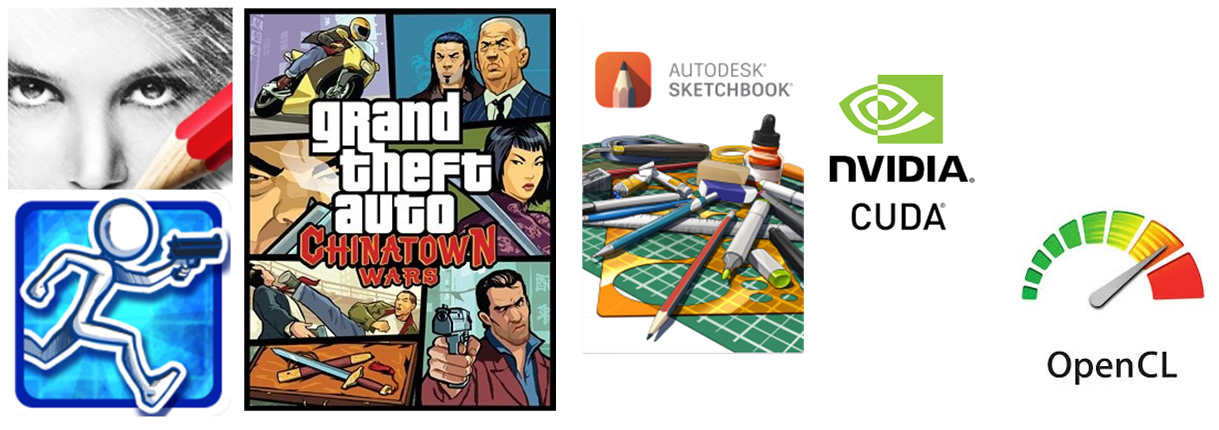
\includegraphics[width=\linewidth]{./figure/background_images.png}
  \end{figure}
\end{frame}

\section{研究内容}
% \section{铅笔画生成算法}
\begin{frame}
  \frametitle{铅笔画生成算法}
  \framesubtitle{基本流程}
  \begin{figure}
    \centering
    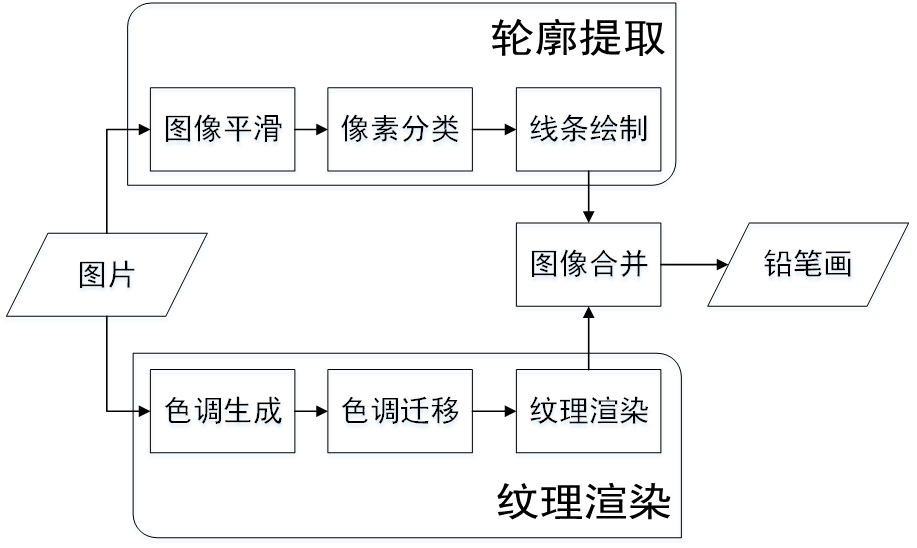
\includegraphics[width=\linewidth]{./figure/alg_flowchart.png}
    % \caption{铅笔画生成算法的流程图}
    % \label{fig:alg-flowchart}
  \end{figure}
\end{frame}

% \section{并行分析与设计}
\subsection{轮廓提取}
\begin{frame}
  \frametitle{并行分析与设计}
  \framesubtitle{轮廓提取}
  \begin{figure}
    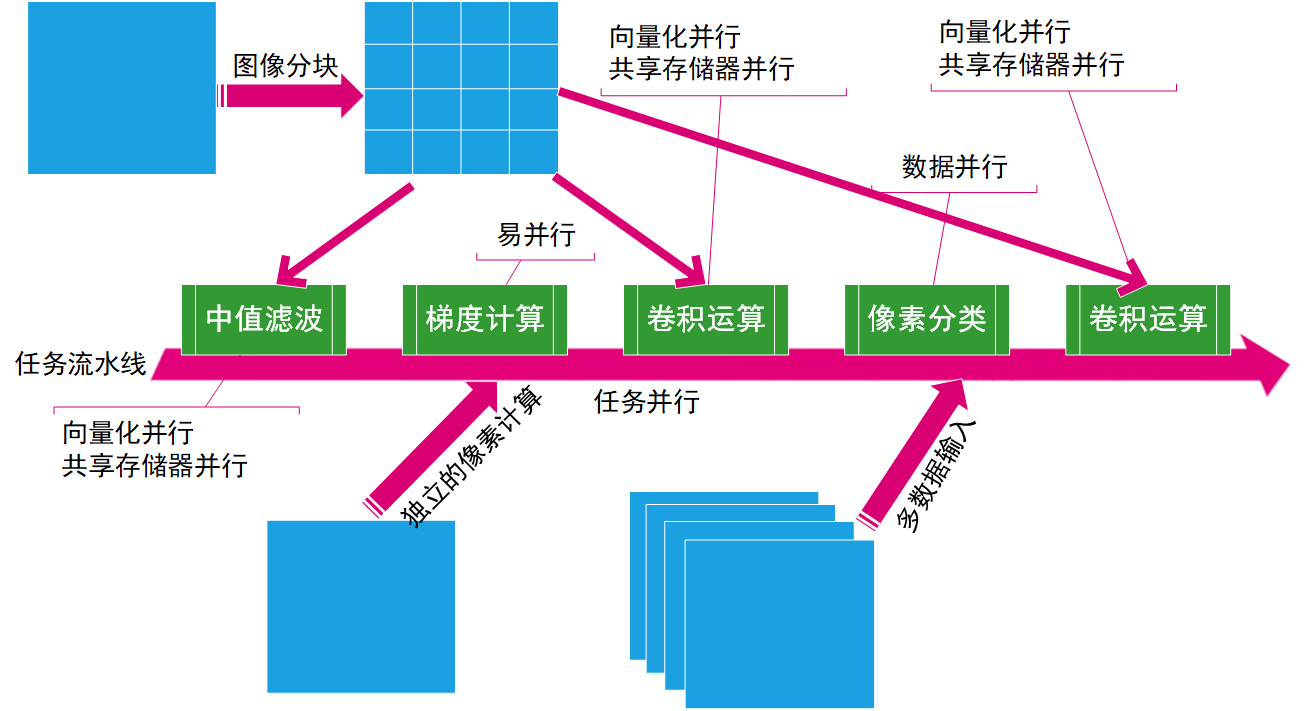
\includegraphics[width=\linewidth]{./figure/ext_stroke_design.png}
    % \caption{}
    % \label{}
  \end{figure}
\end{frame}

% \begin{frame}
%   \frametitle{典型算法设计过程}
%   \framesubtitle{卷积运算}
%   % \begin{figure}
%   %   \includegraphics{/path/to/figure}
%   %   \caption{}
%   %   \label{}
%   % \end{figure}
% \end{frame}

\subsection{纹理渲染}
\begin{frame}
  \frametitle{并行分析与设计}
  \framesubtitle{纹理渲染}
  \begin{figure}
    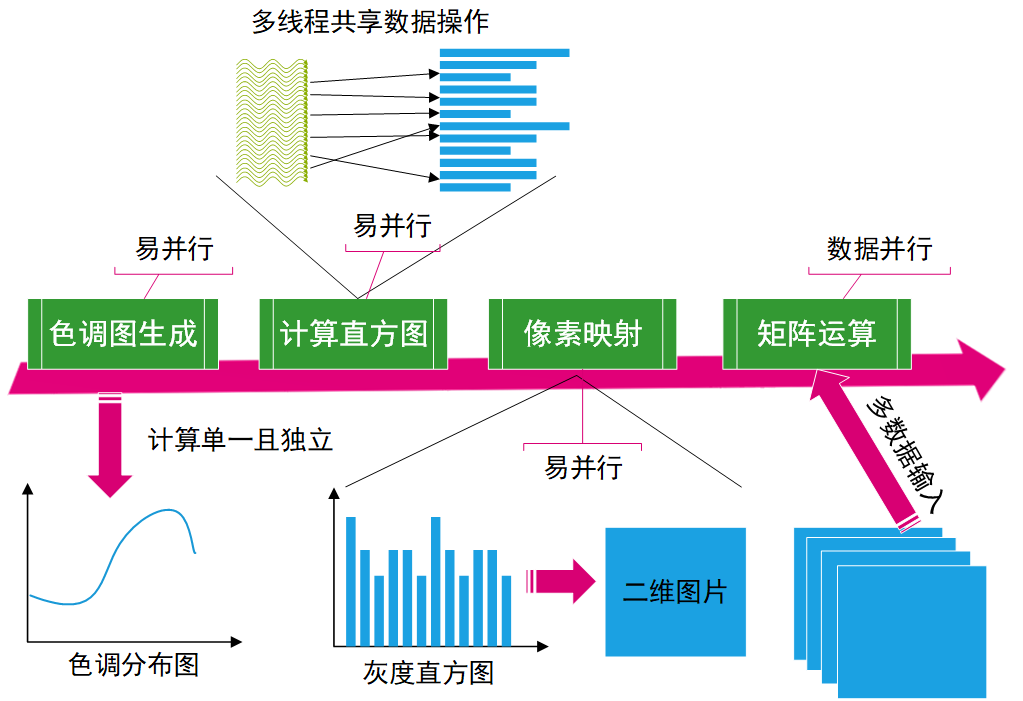
\includegraphics[width=\linewidth]{./figure/texture_render_design.png}
    % \caption{}
    % \label{}
  \end{figure}
\end{frame}

% \begin{frame}
%   \frametitle{典型算法设计过程}
%   \framesubtitle{直方图计算}
%   % \begin{figure}
%   %   \includegraphics{/path/to/figure}
%   %   \caption{}
%   %   \label{}
%   % \end{figure}
% \end{frame}

\subsection{任务级并行}
\begin{frame}
  \frametitle{任务级并行}
  \framesubtitle{任务调度}
  \begin{figure}
    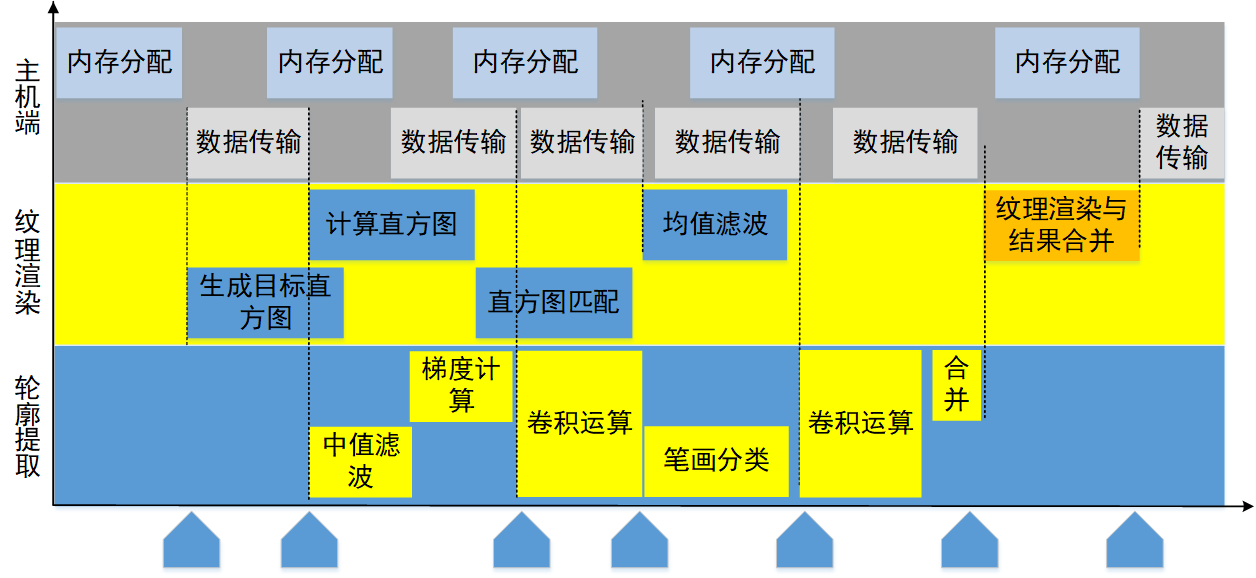
\includegraphics[width=\linewidth]{./figure/task_schedule.png}
    % \caption{任务调度图}
    % \label{}
  \end{figure}
  \begin{block}{说明}
    使用\textrm{CUDA}流技术,对无依赖性的数据计算和数据传输任务重新调度,以实现任务的重叠执行。
  \end{block}
\end{frame}

\subsection{并行实现}
\begin{frame}
  \frametitle{并行实现}
  \framesubtitle{代码仓库}
  \begin{figure}
    \centering
    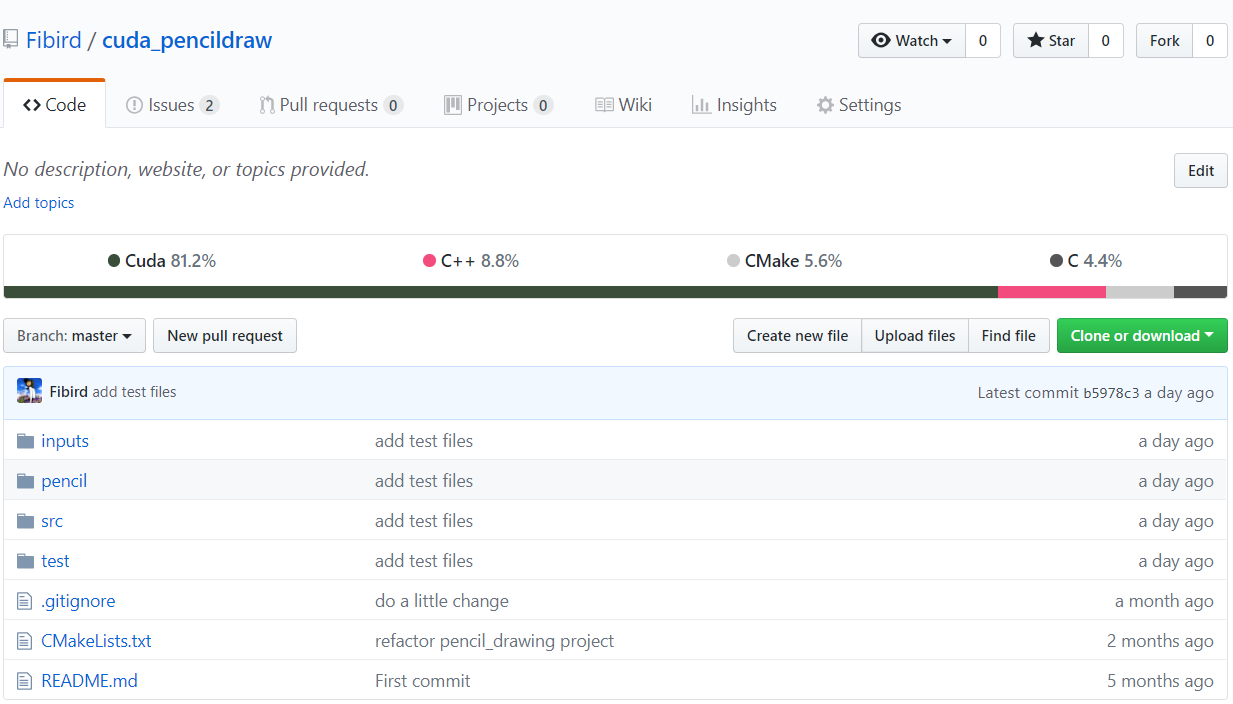
\includegraphics[width=\linewidth]{./figure/code_project.PNG}
    % \caption{}
    % \label{}
  \end{figure}
%   \begin{columns}
%     \begin{column}{0.2\linewidth}
%       \begin{figure}
%         \centering
%         \begin{minipage}[b]{\linewidth}
%           
\includegraphics[width=\linewidth]{./figure/cuda_logo2.jpg}
%         \end{minipage}
%         \begin{minipage}[b]{\linewidth}
%           \includegraphics[width=\linewidth]{./figure/cmake_logo.png}
%         \end{minipage}
%         \begin{minipage}[b]{\linewidth}
%           
\includegraphics[width=\linewidth]{./figure/opencv-logo2.png}
%         \end{minipage}
%       \end{figure}
%     \end{column}
%     \begin{column}{0.8\textwidth}
%       \begin{block}{}
%         算法采用\textrm{CUDA}并行编程模型实现,具有开发周期短,开发效率高等优势;
%       \end{block}
%
%       \begin{block}{}
%         使用\textrm{CUDA runtime API 8.0}实现,采用常量存储器、共享存储器、原子操作等特性;
%       \end{block}
%
%       \begin{block}{}
%         使用\textrm{CMAKE}跨平台的项目构建工具,配置方便,具有跨平台的优势;
%       \end{block}
%
%       \begin{block}{}
%         借助\textrm{OpenCV}计算机视觉库辅助完成图像的解码和编码;
%       \end{block}
%     \end{column}
% \end{columns}
\end{frame}

\section{实验结果与分析}
\begin{frame}
  \frametitle{实验结果与分析}
  \framesubtitle{实验数据集}
  \begin{columns}
    \begin{column}{0.5\linewidth}
      \begin{figure}
        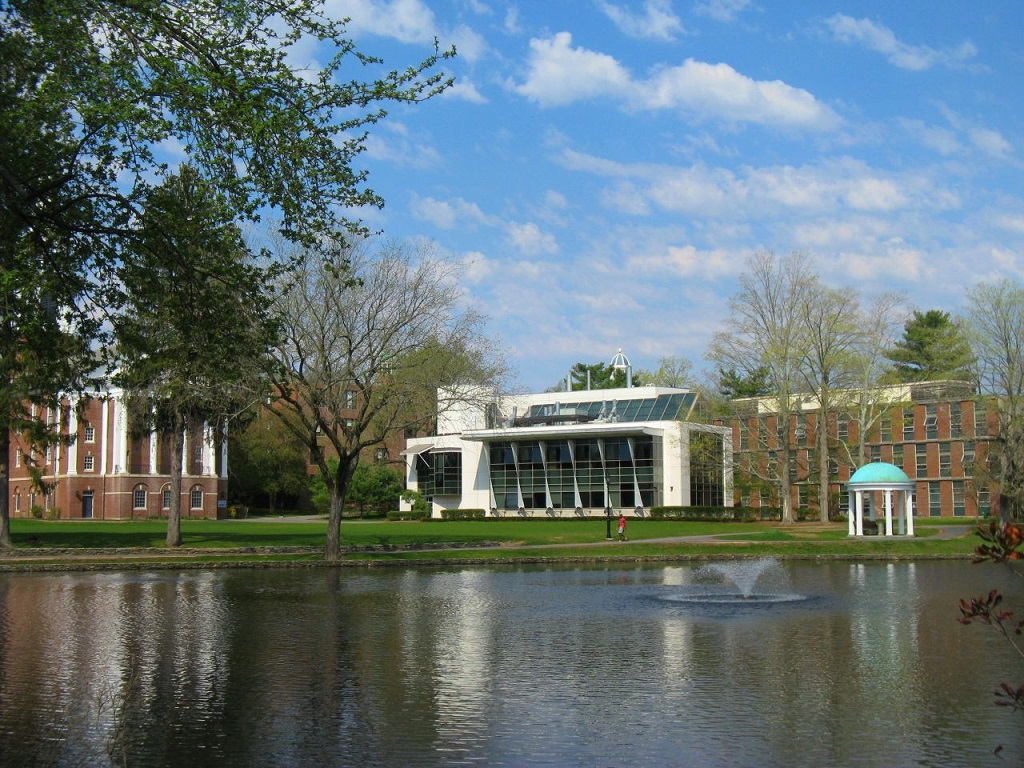
\includegraphics[width=\linewidth]{./figure/test-01.jpg}
        \caption{水波潋滟}
        % \label{}
      \end{figure}
    \end{column}
    \begin{column}{0.5\linewidth}
      \begin{figure}
        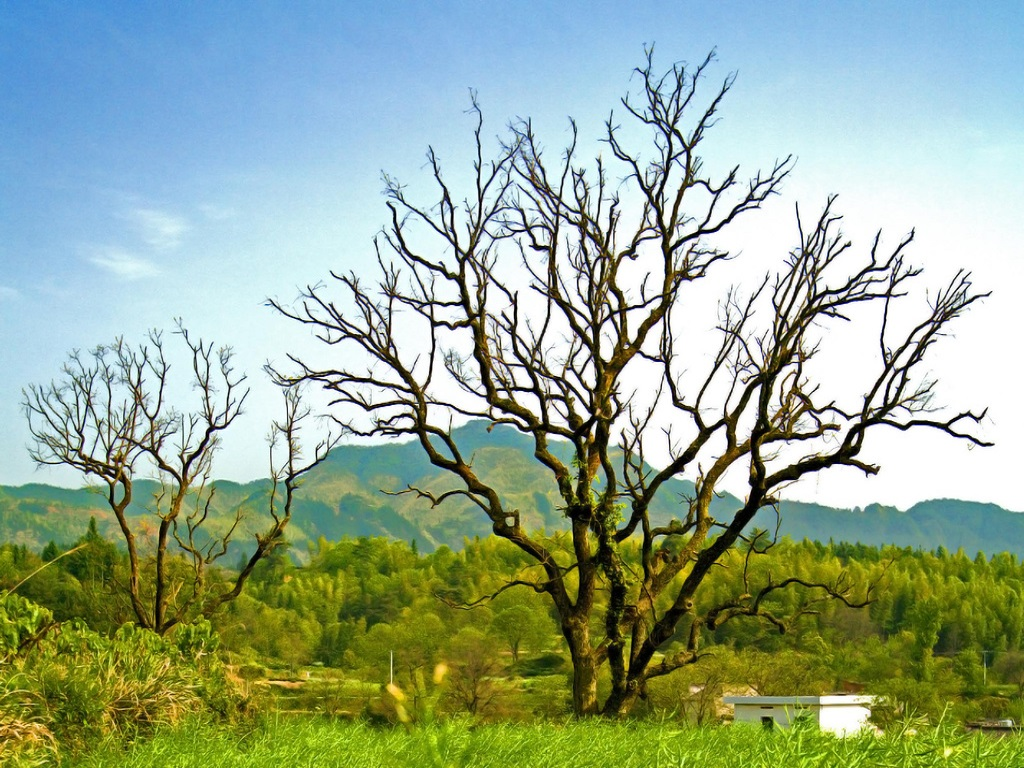
\includegraphics[width=\linewidth]{./figure/test-03.jpg}
        \caption{枯藤老树}
        % \label{}
      \end{figure}
    \end{column}
  \end{columns}
  \begin{block}{注}
    图片来自香港中文大学铅笔画生成算法测试数据集,由于篇幅原因这里只展示两张图片的实验结果。
  \end{block}
\end{frame}

\subsection{算法效果}

\begin{frame}
  \frametitle{实验结果与分析}
  \framesubtitle{算法效果}
\begin{columns}
  \begin{column}{0.5\linewidth}
    \begin{figure}
      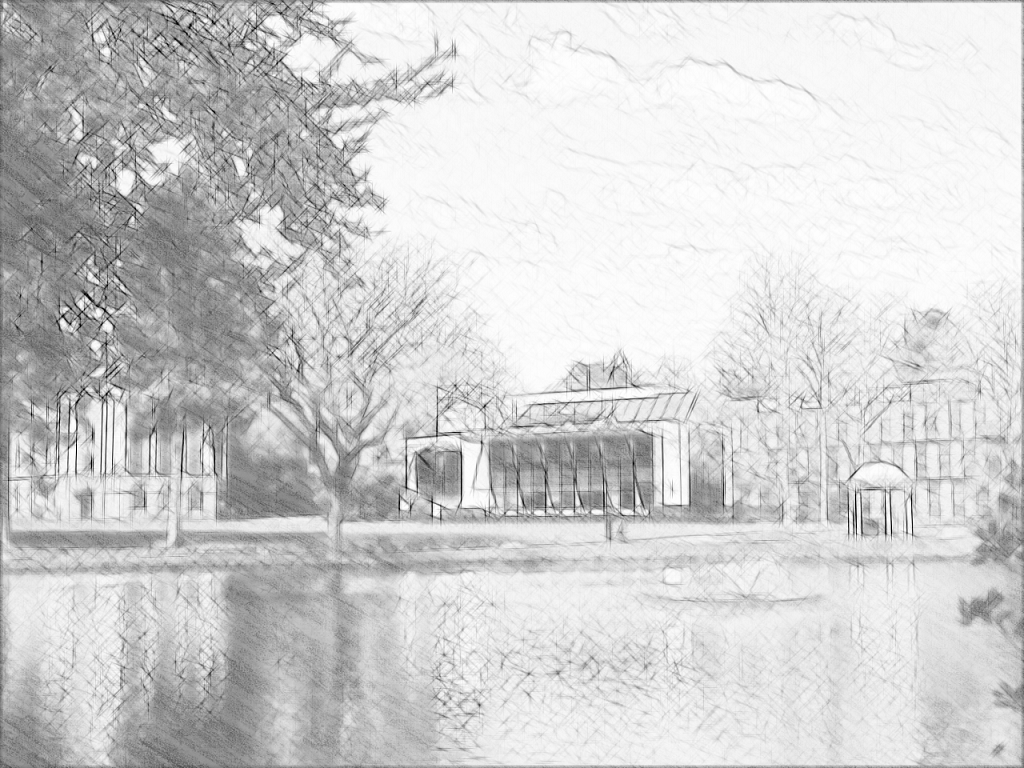
\includegraphics[width=\linewidth]{./figure/thesis_rst-01.png}
      \caption{“水波潋滟”铅笔画结果}
      % \label{}
    \end{figure}
  \end{column}
  \begin{column}{0.5\linewidth}
    \begin{figure}
      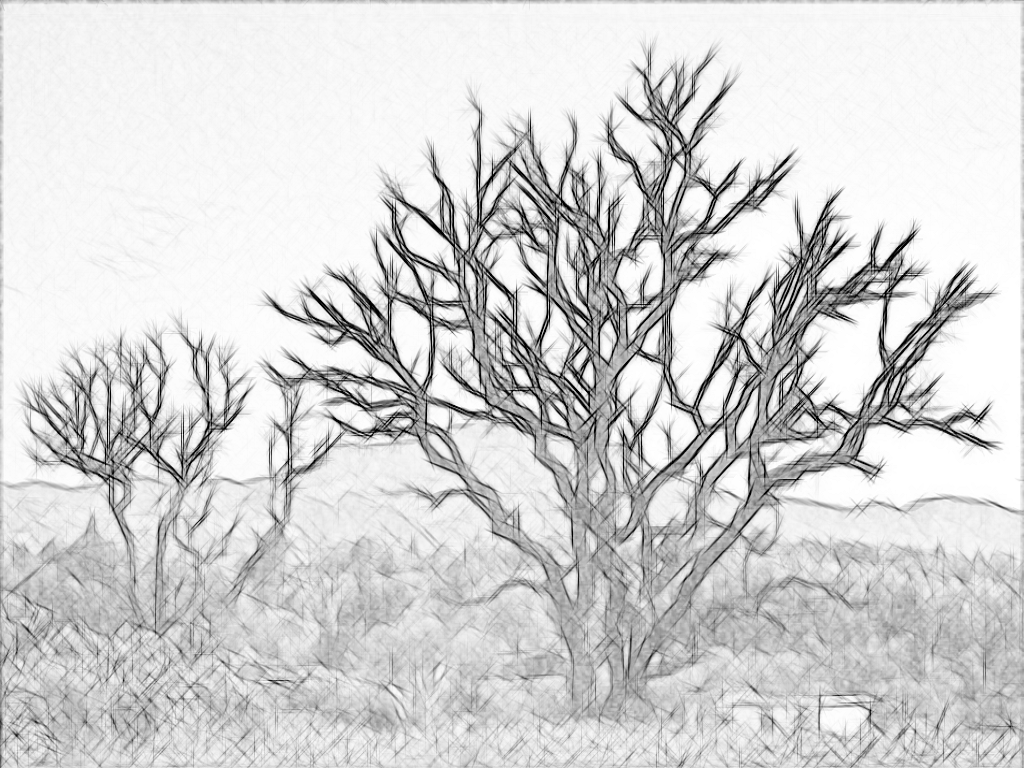
\includegraphics[width=\linewidth]{./figure/thesis_rst-03.png}
      \caption{“枯藤老树”铅笔画结果}
      % \label{}
    \end{figure}
  \end{column}
\end{columns}
\begin{block}{结论}
  处理结果的线条富于变化,具有线条交叉的效果,而且纹理细腻,表现出了铅笔画的光线与阴影效果,比较接近真实的铅笔画。
\end{block}
\end{frame}

\subsection{定量分析}
\begin{frame}
  \frametitle{定量分析指标}
  \framesubtitle{色调分布图}
  \begin{figure}
    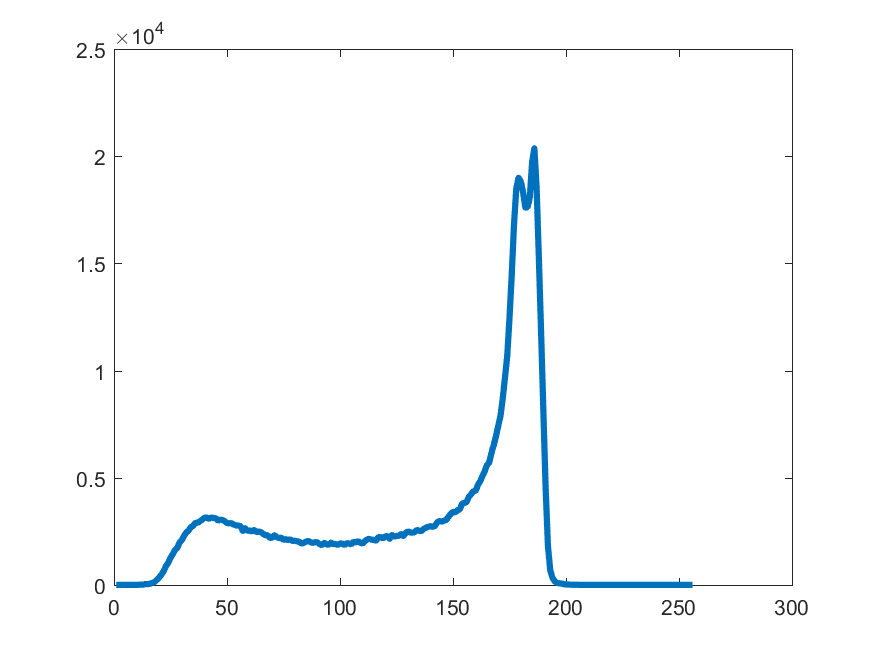
\includegraphics[width=0.6\linewidth]{./figure/sketch_hist-01.png}
    \caption{实际铅笔画色调分布图}
    % \label{}
  \end{figure}
  \begin{block}{}
    \textrm{Li Cewu}等人通过对实际铅笔画的大量分析,建立了实际铅笔画的色调分布模型,如上图所示为该模型的色调分布图。
  \end{block}
\end{frame}

\begin{frame}
  \frametitle{实验结果与分析}
  \framesubtitle{定量分析}
  \begin{columns}
    \begin{column}{0.5\linewidth}
      \begin{figure}
        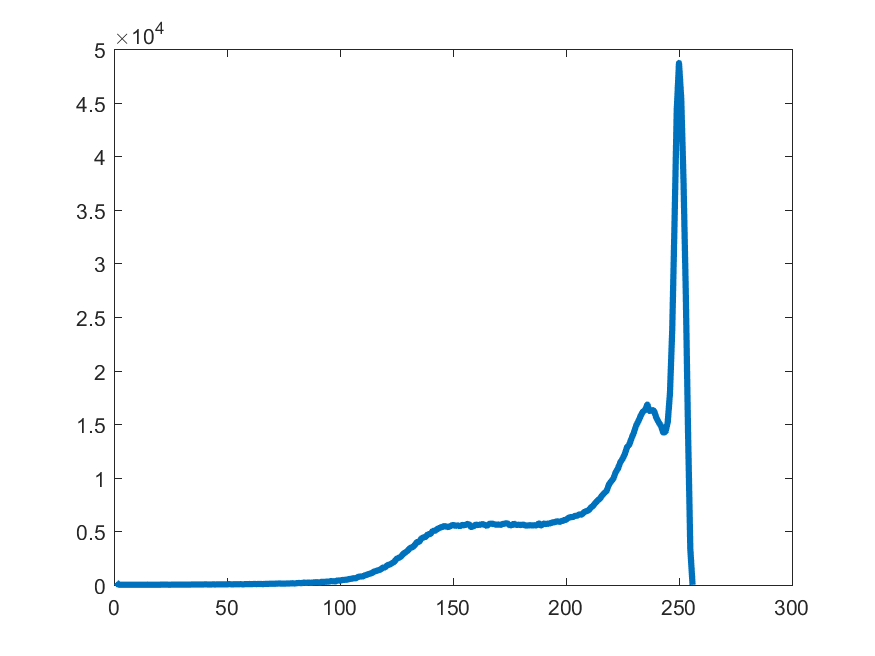
\includegraphics[width=1\linewidth]{./figure/thesis_hist-01.png}
        \caption{“水波潋滟”铅笔画色调分布图}
        % \label{}
      \end{figure}
    \end{column}
    \begin{column}{0.5\linewidth}
      \begin{figure}
        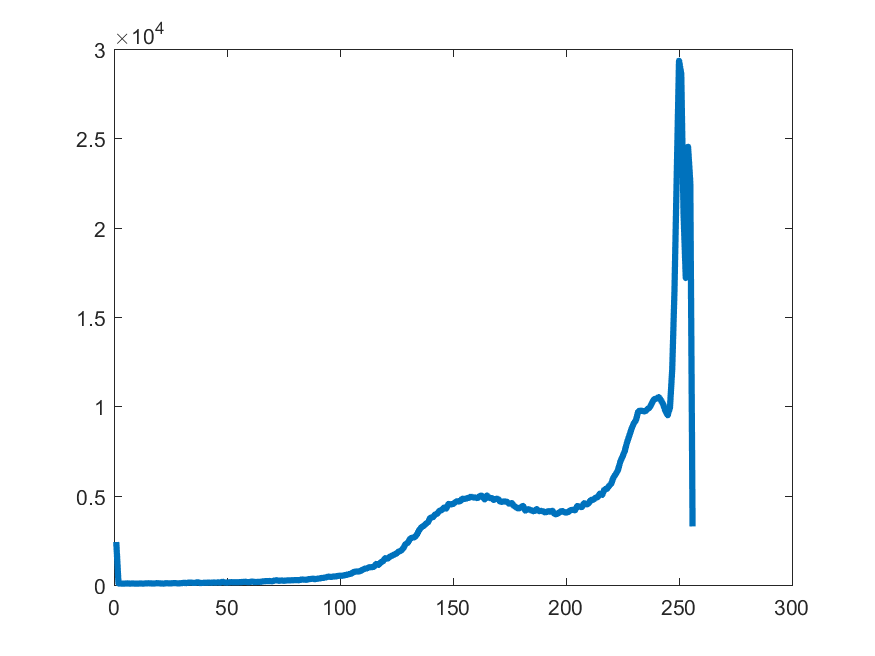
\includegraphics[width=1\linewidth]{./figure/thesis_hist-02.png}
        \caption{“枯藤老树”铅笔画色调分布图}
        % \label{}
      \end{figure}
    \end{column}
  \end{columns}

  \begin{block}{结论}
    本算法生成的铅笔画的色调分布图和实际铅笔画色调分布图的大致相同,因此可以得出本算法生成的铅笔画与实际铅笔画十分接近。
  \end{block}
\end{frame}

\subsection{运行时间与加速比}
\begin{frame}
  \frametitle{实验结果与分析}
  \framesubtitle{运行时间}
  \begin{columns}
    \begin{column}{0.5\linewidth}
      \begin{figure}
        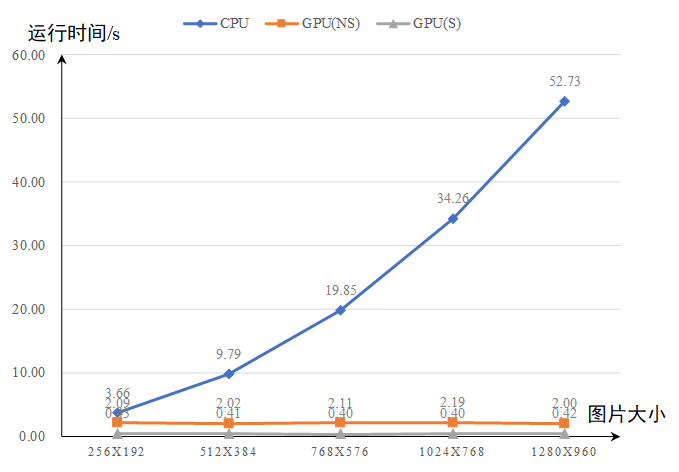
\includegraphics[width=1\linewidth]{./figure/runtime_figure1.png}
        \caption{图“水波潋滟”实验结果}
        % \label{}
      \end{figure}
    \end{column}
    \begin{column}{0.5\linewidth}
      \begin{figure}
        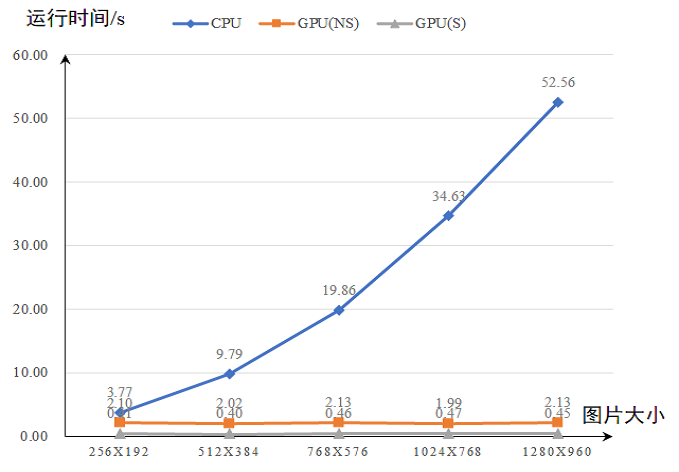
\includegraphics[width=1\linewidth]{./figure/runtime_figure2.png}
        \caption{图“枯藤老树”实验结果}
        % \label{}
      \end{figure}
    \end{column}
  \end{columns}
    \begin{block}{结论}
      \textrm{GPU}并行程序的处理速度远快于\textrm{CPU}串行程序,加速比达10以上,而且运行时间稳定,不受图片大小的影响,满足实时渲染的要求。
    \end{block}
\end{frame}

\begin{frame}
  \frametitle{实验结果与分析}
  \framesubtitle{加速比}
  \begin{table}
    \centering
    \caption{两种GPU算法的平均加速比}
    \begin{tabular}{ccc}
      \toprule[1pt]
         图片大小 & \textrm{GPU(No-Stream)} & \textrm{GPU(Stream)}	\\
      \midrule
      256x192	&1.78&	9.23 \\
      512x384	&4.68&	22.53 \\
      768x576	&9.32&	44.50 \\
      1024x768 &	16.22&	80.59 \\
      1280x960	& 25.15&	120.32 \\
      \bottomrule[1pt]
    \end{tabular}
  \end{table}
  \begin{block}{结论}
    使用\textrm{CUDA}流技术的\textrm{GPU}算法的加速比大于未使用\textrm{CUDA}流的算法,前者大概为后者的5倍左右,因此使用\textrm{CUDA}流技术可以大大加快程序运行速度。
  \end{block}
\end{frame}

\section{总结与展望}
\begin{frame}
  \frametitle{总结与展望}
  \framesubtitle{}
  \begin{block}{总结}
    本文针对目前铅笔画生成算法实时效果差的问题,提出了一种基于CUDA的并行快速铅笔画生成算法,这种算法不仅可以获得逼真的铅笔画效果,而且处理速度快,满足实时渲染的要求,在游戏、动画等领域具有广泛的应用前景。
  \end{block}
  \begin{block}{展望}
    目前本算法只能生成单色调铅笔画,可以将算法适当改进以实现彩色铅笔画的生成。
  \end{block}
\end{frame}

{
\nwsuafwavesbg
  \begin{frame}[plain,noframenumbering]
    \finalpage{感谢您的聆听!\\欢迎多提宝贵意见和建
      议!}
  \end{frame}
}
%%%%%%%%%%%%%%%%
\end{document}

%%% Local Variables:
%%% mode: latex
%%% TeX-master: t
%%% End:
